\documentclass[10pt]{article}
\usepackage[margin=0.7in]{geometry}\usepackage[T1]{fontenc}\usepackage{lmodern,amsmath,amssymb,graphicx,booktabs,microtype,hyperref}
\setlength{\parindent}{0pt}\setlength{\parskip}{5pt}
\begin{document}
{\LARGE Signed two-summand rank}\par
{\large Finite census and a checked dependency mechanism}\par
2026-10-29 \quad PR2381 \quad Native counts, not a speed result

\textbf{Question.} Does the complete signed two-summand S3 row model constrain
empty-state useful rank? The lead atlas already records raw decomposition
conservation (KN-FIND-007); row independence is a separate question.
The original twist yield/degree/main-source-DLP objective remains open.

\textbf{Exact finite population.} Odd primes $r=3,5,7,11,13,17,19,23,29,31$;
all $1\le b\le\min(4,(r-1)/2)$ subsets of sign representatives; every nonzero
query, complete two-summand rows, coefficients in $\mathbf F_r$.
C++ ordered enumeration and independent Rust unordered construction agree on
\textbf{4,485 bases,119,912 queries,zero rank/count defects}.
These are abstract cyclic bases, not elliptic models.

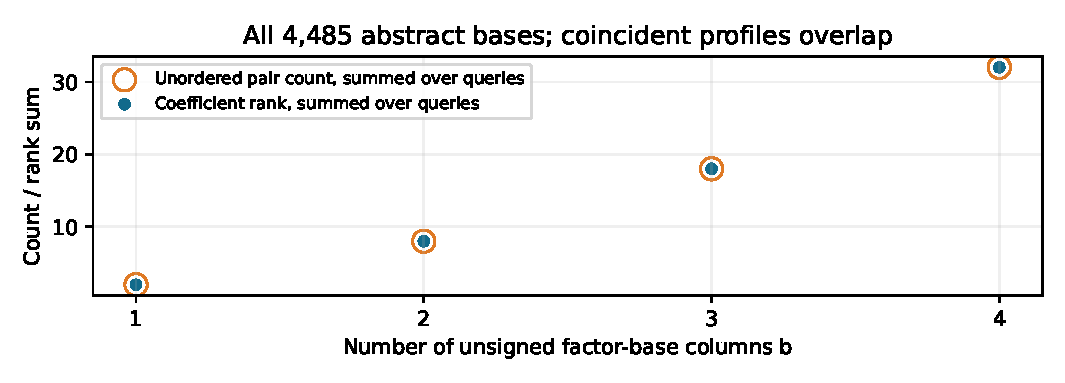
\includegraphics[width=\linewidth]{profiles.pdf}
All recorded bases plotted; overlapping profiles coincide. No sampling interval.
Full rows are reconstructed independently and bound by exact stream hashes.

Both paths also match every row of the \textbf{96 frozen actual S3 arms /896queries}
on the prior F43/r11 and F13/r7 source reductions. This checks old point-row
bindings; it is not a new scalar-recovery experiment. All failures and policies
remain in the frozen source records.

\begin{center}\begin{tabular}{llll}\toprule
Domain control & Target & Rank & Pair count\\\midrule
$\mathbf Z/9$,base $\{1,2,4\}$,coefficients $\mathbf F_{101}$ &3&2&3\\
$\mathbf Z/7$,base $\{1\}$,coefficients $\mathbf F_2$ &2&0&1\\\bottomrule
\end{tabular}\end{center}
The first removes target generation. The second loses the diagonal factor2.
These retained losses prevent extending the finite observation without assumptions.

\textbf{Validation.} Both full native attempts pass;six changed/rehashed
corruptions reject101/no receipt;22backend tests pass. The second attempt changes
only the Lean-source binding after a simplification fix; all case/profile bytes
and audit receipts match. No time,GAE,S,regularity or practical advantage claim.
\newpage
{\LARGE Checked kernel, open matrix bridge}\par
Five public named theorems /five audited declarations; zero failing or extra
trusted axioms under the unmodified scoped repository proof gate. Only
\texttt{propext,Classical.choice,Quot.sound}. Lean4.34.1/Mathlibd13f23b7.

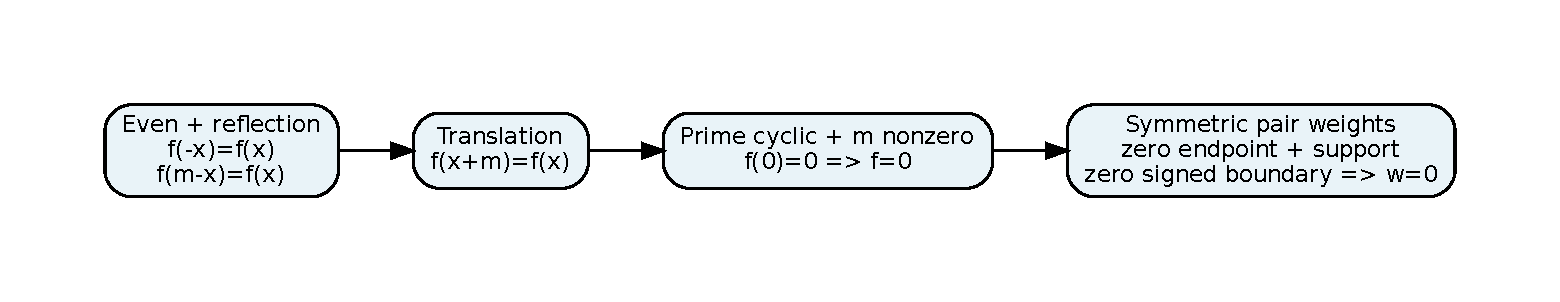
\includegraphics[width=\linewidth]{bridge.pdf}

For prime $r$,nonzero $m\in\mathbf Z/r$,an even function with
$f(m-x)=f(x)$ and $f(0)=0$ is zero: symmetry gives translation by$m$ and
multiples of$m$ exhaust the group. For symmetric pair weights supported on
$x+y=m$,zero at endpoint0,zero signed boundary therefore implies zero weights.
These support and balance equations are written hypotheses.

\textbf{Open formal binding.} This is not yet a universal theorem that every
signed coefficient-row family is independent. Diagonal weight conversion needs
$2\ne0$; the general actual matrix-family binding and combinatorial count remain
unformalized. The native census separately checks actual matrices in its bounds.
Known raw counting would yield $2b^2/(r-1)$ mean rank \emph{if} that complete
independence binding holds. The18th source-bound IDC1 record checks only
$(2b)(2b+1)-2b=4b^2$,32+16native points,with false-identity/source controls;
it certifies neither independence nor speed.

\textbf{Honest flow.} Protocol/source were committed before main data. A declared
one-call pilot precedes canonical JSON freeze; no threshold/population changed.
Canonical protocol hash begins\texttt{a89bfebc5982a78e};checker from atlas8b8800af.
Two full native contracts completed,zero excluded/interrupted/resumed; repeated
outputs are not independent samples. First actual Lean build failed on
$f(0)=w(0,m-0)$ simplification; same theorem fixed and final gate passes.
The original failed source/log remains,including its unaccepted sorry axiom.
Export validation caught a pilot-only CLI guard added after the analysis hash.
Exact frozen analyzer bytes were restored and both output sets replayed;the
frozen protocol/hash was not rewritten. Missing JSON serializer and absent timing utility are separate infrastructure
failures. No frozen prior source was patched.

\textbf{What remains.} A twist advantage in relevant degree/complete work,
stationary useful yield,actual-state probability,broader geometry and full
calibration remain open. Root5140-case library validation is still incomplete
at600sec/124; naming/1921missing study registrations,required CI,coordination and
integration remain held. No registry,benchmark or leaderboard row changed.
No new speedup,universal impossibility,hardness,GHS or invalid-curve claim.

\textbf{Reproduce.} See adjacent README for exact protocol,source files,native
runner,scoped Lean gate,byte-part case restoration and raw restoration. Native
caps600sec;bounded iteration23:23--00:23UTC;two localworkers,no paidcompute.
Approved branch checkpoint access works;credentials are outside Git/evidence.
The next step must bind a useful actual matrix/probability result or a new
relevant-degree encoding,while preserving the original main-source DLP goal.

\small Sources: frozen uniform/S3 and CM8/dual reports;Mathlib ZMod;lead-atlas
KN-FIND-007,relation-graph-rank and Semaev-yield leads. Full source and retained
failures linked in README. All numbers above copy native/audit records.
\end{document}
